% -----------------------------------------------------------------------------
% Fundamentals
% -----------------------------------------------------------------------------
\chapter{Fundamentals}
\label{chap:fundamentals}
In order to be up to snuff on how a \textit{spatial ANC} system works some understanding in acoustics is compulsory e.g. how to model a sound source, how the wave emitted by this source propagates in a 3-dimensional room i.e. how the wave is reflected by the rooms walls.\\
Albeit there's multiple means of implementing \textit{spatial ANC} this paper will only carry out one possible implementation \textit{quod est} the wave-domain least mean square algorithm which requires for the acoustic model to be modeled in the wave domain which has proven to be the most challenging segment but in return simplifies the process of \textit{spatial ANC}.

\section{Propagation of sound}
An acoustic wave is essentially a change in pressure. A local pressure change causes the surrounding medium to compress which in turn causes pressure changes thus leading to the propagation of an acoustic wave. This compression leads to a displacement of the particles in the medium.\\The linear wave equation can be used to describe such an acoustic wave. In reality the acoustic wave equation is non linear but for this application the linear approximation to the wave equation is a good model.\cite{Acoustic}\\
\subsection{Linearity}
Viewing acoustics as a linear phenomenon is very appealing due to the principle of superposition roughly depicted by following relation
\begin{equation}
    \mathcal{L}(af_1+bf_2) = a\mathcal{L}(f_1) + b\mathcal{L}(f_2),
\end{equation}
where
$f_1$ and $f_2$ are two causes,\\
$\mathcal{L}(f)$ is the set of possible computational steps that predict the effect of $f$.\\
Thus a complex sound field stemming from multiple sources can be regarded as the sum of sound fields produced by each source individually. In the same way a complex wave can be analyzed by each frequency separately. Nevertheless this acoustic model only represents an approximation\cite{Rossing2007}.\\
\\
The following three laws are used to develop the wave equation.
\subsection{Equation of State}
The equation of state relates changes in pressure and density. It is determined by thermodynamic properties and dependant upon the material. The equation of state for linear acoustic waves in fluid is  given by\cite{Acoustic}
\begin{equation}
    p = \mathbf{B}s = \rho_0c^2s,
\end{equation}
where 
$\mathbf{B}=\rho_0(\frac{\partial P}{\partial \rho})_{\rho_0}$ is the adiabatic bulk modulus,\\
$\rho$ in $kg/m³$ is the density,
$\rho_0$ is the undisturbed density,\\
$p$ in $Pascal$ where $1Pa = 1 N/m^2 = 1kg/s^2/m$ is the pressure,\\
$P$ is the instantaneous pressure,\\
$c$ in $m/s$ is the speed of sound,\\
$s = \frac{\rho-\rho_0}{\rho_0}$ is the condensation 
\subsection{Equation of Continuity}
The equation of continuity depicts the conservation of mass:
\begin{equation}
    \frac{\partial\rho}{\partial t} = -\rho_0\nabla\cdot\Vec{u},
\end{equation}
where\\
$t$ is time,\\
$\nabla$ is the Nabla operator.\\
$\Vec{u} = \frac{\partial\Vec{\xi}}{\partial t}$ is the particle velocity,\\
$\Vec{\xi}$ is the particle displacement,\\
$\Vec{x}$ is the particle position.
\subsection{Equation of Motion}
The Equation of motion describes how a pressure variation generates a force that causes particle motion:
\begin{equation}
    -\nabla p = \rho_0 \cdot \frac{\partial\Vec{u}}{\partial t}
\end{equation}
\subsection{Wave Equation}
The wave equation or the equation of propagation of acoustic pressure can be derived from the three preceding equations:
\begin{equation}
    \frac{1}{c^2}\frac{\partial^2p}{\partial t^2} = \nabla^2p
\end{equation}
in Cartesian coordinates $(x,y,z)$:
\begin{equation}
    \frac{1}{c^2}\frac{\partial^2p}{\partial t^2} = \frac{\partial^2p}{\partial x^2} + \frac{\partial^2p}{\partial y^2} + \frac{\partial^2p}{\partial z^2},
\end{equation}
in Polar coordinates $(r,\theta, z)$:
\begin{equation}
    \frac{1}{c^2}\frac{\partial^2p}{\partial t^2} = \frac{\partial^2p}{r^2\partial \theta^2} + \frac{\partial^2p}{\partial r^2} + \frac{1}{r}\frac{\partial^2p}{\partial r} + \frac{\partial^2p}{\partial z^2},
\end{equation}

\subsection{Spherical Wave Equation}

For simplicity we assume the acoustic source to be a point source, it can thus be represented as a spherical wave. Furthermore we assume "spherical symmetry" i.e. the pressure and particle velocity are equal for the same $r$, the distance from the 'origin' of the spherical wave. The wave equation for the spherically symmetric wave is\cite{Waves2004}:
\begin{equation}
    \frac{\partial^2rp(r,t)}{\partial r^2} = \frac{1}{c^2}\frac{\partial^2rp(r,t)}{\partial t^2}.
\end{equation}
\subsubsection{General Solution to the Spherical Wave Equation}
A general solution to the wave equation is given by the pressure wave emitted by a single frequency point source of acceleration in free space\cite{Allen1979}:
\begin{equation}
    p(\omega,\Vec{x},\Vec{x}') = \frac{e^{i\omega(\frac{r}{c}-t)}}{4\pi r}\quad\quad for\quad r > 0,
\end{equation}
where\\
$p$ is the pressure,\\
$\omega=2\pi f$,\\
$f$ is the frequency,\\
$r=|\Vec{x}-\Vec{x}'|$ is the distance from source to receiver,\\
$\Vec{x}$ is the source location $(x,y,z)$,\\
$\Vec{x}'$ is the receiver location $(x',y',z')$,\\
$i=\sqrt{-1}$.\\


\section{Spherical Harmonics}
To implement the wave-domain least square method the acoustic model needs to be implemented in the wave domain thus requiring a representation of the primary and secondary noise field by the means of spherical harmonics.
"The spherical harmonics are a set of orthogonal spatial basis functions that can be utilized
to decompose any arbitrary function defined on the sphere."\cite{Samarasinghe2018}\\ A graphical representation of spherical harmonics can be seen in \textit{figure \ref{fig:sph_harmonics}}.\\
\begin{figure}
    \centerline{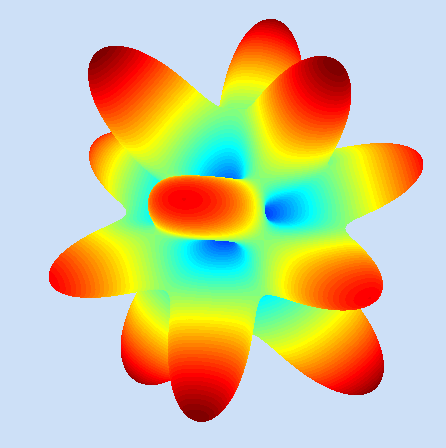
\includegraphics[width=1.3\textwidth,keepaspectratio]{LaTeX/images/plots/spherical_hamonics.png}}
    \caption{visualization of surface spherical harmonic functions of degree 6 and order 3 generated by Dimitrios Piretzidis (2022). Surface Spherical Harmonic Functions Visualization (https://www.mathworks.com/matlabcentral/fileexchange/44869-surface-spherical-harmonic-functions-visualization)}
    \label{fig:sph_harmonics}
\end{figure}
A homogeneous incident wave field $v(\mathbf{x},k)$ observed at $\mathbf{x}$ can thus be decomposed into\cite{Zhang2019}:
\begin{equation}
    v(\mathbf{x},k)=\sum_{u=0}^\infty \sum_{m=-u}^u\beta_{um}(k)j_u(kr)Y_{um}(\theta_x,\phi_x),
    \label{eq:wave_field_decomposition}
\end{equation}
for any location with spherical coordinates $\mathbf{x}=(x,\theta_x,\phi_x)$\\\\
where\\
$\theta = tan^{-1}\bigg(\frac{\sqrt{x^2+y^2}}{z}\bigg)$ is the elevation angle from $0$ to $\pi$,\\
$\phi = atan2\bigg(y,x\bigg) = tan^{-1}\bigg(\frac{y}{x}\bigg),\quad  x >0$ is the azimuth angle from $0$ to $2\pi$,\\
$k=2\pi f/c$ is the wave number,\\
$f$ is the frequency,\\
$c$ is the speed of sound,\\
$j_u(.)$ is the spherical Bessel function of order $u$,\\
$\beta_{um}(k)$ is the harmonic coefficient.\\ 
$Y_{um}(.)$ is the spherical harmonics,\\
The spherical harmonics function of order $n$ and mode $m$ is defined by\cite{Samarasinghe2018}
\begin{equation}
    Y_{um}(\theta_x,\phi_x) = \mathbf{P}_{n|m|}(cos(\theta_x))\frac{1}{\sqrt{2\pi}}e^{im\phi_x},
\end{equation}
where\\
$\mathbf{P}_{n|m|}(cos(\Phi_x))$ is the associated Legendre polynomials.\\\\
Finding the appropriate harmonic coefficients will be necessary to define the noise field in the wave-domain.
\subsection{Plane Wave Expansion in Spherical Harmonics}
A plane wave can be expressed as a linear combination spherical harmonic waves\cite{Mehrem2011}:
\begin{equation}
    e^{i\mathbf k \cdot \mathbf r} = 4 \pi \sum^\infty_{l=0}\sum_{m=-l}^l i^lj_u(kr)\overline Y_{um}(\mathbf \hat k){Y}_{um}(\mathbf \hat r),
    \label{eq:plane_wave_expansion}
\end{equation}
where\\
$\overline Y_{um} = (-1)^mY_{l,-m}$ is the complex conjugate matrix,\\
$i$ is the imaginary unit,\\
$\mathbf k$ is a wave vector of length $k$,\\
$\mathbf r$ is a position vector of length $r$,\\
$\mathbf{ \hat{k}} = \frac{\mathbf{k}}{|\mathbf k|}$ and $\mathbf{\hat{r}}$ is the unit vector of $\mathbf k$ and $\mathbf r$ respectively.\\
in spherical coordinates $\mathbf k\{k,\theta_k,\phi_k\}$ and $\mathbf r\{r,\theta_r,\phi_r\}$:
\begin{equation}
    e^{i \mathbf k \cdot \mathbf r} = 4 \pi \sum^\infty_{l=0}\sum_{m=-l}^l i^lj_u(kr)\overline Y_{um}(\theta_k,\phi_k){Y}_{um}(\theta_r,\phi_r),
\end{equation}
where\\
$\mathbf k \cdot \mathbf r = kr[\sin\theta_k\sin\theta_r\cos(\phi_k-\phi_2)+\cos\theta_k\cos\theta_r]$,\\
$k = \frac{2\pi}{\lambda} = \frac{2\pi f}{c}$,\\
$\lambda$ is the wave length.\\\\
Substituting \ref{eq:plane_wave_expansion} into \ref{eq:wave_field_decomposition} yields\\
\begin{flalign}
\begin{split}
    4\pi i^lj_u(kr)\overline Y_{um}(\theta_k,\phi_k){Y}_{um}(\theta_r,\phi_r) & = \beta_{um}(k)j_u(kr)Y_{um}(\theta_r,\phi_r)\\
    \Leftrightarrow \beta_{um}(k) & = 4\pi i^l  \overline Y_{um}(\theta_k,\phi_k)\frac{{Y}_{um}(\theta_r,\phi_r) }{Y_{um}(\theta_r,\phi_r)}\\
    \Leftrightarrow \beta_{um}(k) & = 4\pi i^l  \overline Y_{um}(\theta_k,\phi_k)
\end{split}
\end{flalign}\\
resulting in an exact solution of the harmonic coefficients for a plane wave.\\\\
\textit{Nota}\\
The plane wave expansion is studied in order to compare its exact solution to the approximated result provided by the implementation of the general equation.

\subsection{Harmonic Coefficients}
When multiplying both sides of \ref{eq:wave_field_decomposition} by $\overline Y_{um}$ and integrating over the sphere with radius $R$ we get\cite{Chen2017}:\\
\begin{equation}
    {\beta_{um}(k) = \frac{1}{\mathbf j_l(kR)}\int_0^\pi\int_0^{2\pi}P(R,\theta,\phi,k) \overline {\mathbf{Y}}_{um}(\theta,\phi)\,d\theta\, d\phi}
    \label{eq:harmonic_coefficients}
\end{equation}\\
For a given pressure signal this equation cannot be solved analytically, a numerical approximation is necessary.
\section{Spatial Sound Recording using a Spherical Microphone Array}
Capturing the harmonics coefficients for the entire room with a limited amount of microphones is inconceivable. This however is not paramount as only a region within the room, the quiet zone, is of interest. In order to record the harmonic coefficients a spherical microphone array is placed around the region of interest. The use of a \textbf{spherical} microphone array is convenient due to its geometry coinciding with that of the spherical harmonics\cite{Chen2017}.\\
To define the position of the microphones on the sphere a sampling method is required.
\subsection{Gauss-Legendre Quadrature on the Sphere}
The spherical harmonic transform from \ref{eq:harmonic_coefficients} can be sampled using the Gaussian sampling scheme and is given by
\begin{equation}
    \beta_{um}(k) = \frac{1}{j_l(kR)} \sum_{q=0}^N\sum_{p=0}^{2N+1}a_qP(R,\theta_q,\phi_p,k)\overline Y_{um}(\theta_q,\phi_p),
\end{equation}
where the weights are
\begin{equation}
    a_q = \frac{\pi}{N+1}\frac{2(1-\cos^2\theta_q)}{(N+2)^2[P_{N+2}(\cos \theta_q)]^2}, \quad 0 \leq q\leq N
\end{equation}
The azimuth angle is sampled at $2(N+1)$ equal-angle samples:
\begin{equation}
    \phi_p = p\frac{2\pi}{2N+2},\quad p=0,...,2N+1
\end{equation}
and the elevation angle is sampled by selecting $(N+1)$ samples that are the zeros of $P_{N+1}(\cos\theta)$:
\begin{equation}
    P_{N+1}(\cos\theta_q)=0, \quad 0 \leq q \leq N
\end{equation}
where\\
$P_{N+1}$ is the Legendre polynomial of degree $N+1$\\\\
which results in a total number of samples \textit{ergo} microphones of $2(N+1)^2$\\\\
The advantage of the Gaussian sampling scheme is its relative low number of sample point compared to other sampling methods such as the equal-angle sampling scheme\cite{Rafaely2015}.\\\\
An appropriate microphone setup should yield a set of harmonic coefficients resulting in a decent representation of the primary sound field emitted by the noise source observed within the region of interest. These coefficients can subsequently be used to generate a secondary \textit{anti noise} sound field.

\section{Spatial Active Noise Control}
The process of \textit{spacial ANC} seeks to reduce the residual signal at any point $\mathbf{x} \equiv \{r,\theta_x, \phi_x$ within the region of interest. The residual signal is given by
\begin{equation}
    e(\mathbf{x},k) = v(\mathbf{x},k) + s(\mathbf{x},k),
\end{equation}
where\\
$k$ is the wave number,\\
$v(\mathbf{x},k)$ is the primary noise field observed at a point $\mathbf{x}$ i.e. the noise field generated by noise source and its reverberation in the room.\\
$s(\mathbf{x},k)$ is the secondary noise field i.e. the \textit{anti-}noise field emitted by the set of loudspeakers on behalf of the ANC process.
\subsection{Primary Noise Field}
The primary noise field can be expressed using the spherical harmonics decomposition in \ref{eq:wave_field_decomposition}. Within the region of interest the noise field can be approximated with a finite number of modes with truncation order of $N = \lceil ekR_1/2\rceil$ 


\subsection{Secondary Noise Field}
Applying a simple loudspeaker model the secondary noise field can be represented by \cite{Zhang2019}
\begin{equation}
    s(\mathbf{x},k) = 
\end{equation}

\section{Simulating an acoustic source in 3D - space}
Once again there's multiple ways of modeling the reverberation of an acoustic source in a 3-dimentional room such as ray/beam tracing, boundary and finite element methods and digital waveguide meshes be as it may this paper resorts to the approach outlined by Allen and Berkley in 1979 which due to its simplicity and adequate accuracy still remains a sought-after technique \cite{Samarasinghe2018}

\subsection{Image Source Method}
The image model is a method that allows the computation of a source-to-receiver acoustic transfer function in an enclosed 3D-space. Within this method an acoustic wave produced by a source, when crossing a wall, produces an image which then itself is considered as a source for further computation. In a room with several walls each image then also produces an image.\cite{Allen1979}
\\\\
The exact solution to the wave equation in a rectangular, rigid-wall, room is given by the rooms impulse response function also known as the time domain Green's function\cite{Allen1979}:
\begin{equation}
    p(t,\mathbf{X},\mathbf{X'})=\sum_{p=1}^8\sum_{r=-\infty}^\infty\frac{\delta[t-\frac{|\mathbf{R_p}+\mathbf{R_r}|}{c}]}{4\pi|\mathbf{R_p}+\mathbf{R_r}|},
\end{equation}
where\\ 
$c=$ the speed of sound,\\
$\mathbf{R_p}$ represents the eight vectors given by the eight permutations over $\pm$ of
\begin{equation}
    \mathbf{R_p}=(x\pm x', y\pm y', z\pm z')
\end{equation}
r is the integer vector triplet $(n,l,m)$, and
\begin{equation}
    \mathbf{R_r}=2(nL_x, lL_y, mL_z),
\end{equation}
where $(L_x, L_y, L_z)$ are the room dimensions.
\\
\\
In case of non-rigid walls, the solution to the wave equation becomes more complicated and is only conceivable under the assumption that the wall impedance is proportional to $sec(\theta)$, where $\theta$ is the angle incidence of a plane wave with respect to the wall normal, resulting in the Sabine energy absorption coefficient $\alpha$ for a uniform reflection coefficient $\beta$ on a given wall of the form\cite{Allen1979}:
\begin{equation}
    \alpha=1-\beta^2.
\end{equation}
The modified room impulse response transforms into:
\begin{equation}
    p(t,\mathbf{X},\mathbf{X'})=\sum_{p=1}^8\sum_{r=-\infty}^\infty
    \beta_{x1}^{|n-q|}\beta_{x2}^{|n|}\beta_{y1}^{|i-j|}\beta_{y2}^{|i|}\beta_{z1}^{|m-k|}\beta_{z2}^{|m|}
    \frac{\delta[t-\frac{|\mathbf{R_p}+\mathbf{R_r}|}{c}]}{4\pi|\mathbf{R_p}+\mathbf{R_r}|},
\end{equation}
where\\
$p=(q,j,k)$ and $r=(n,l,m)$ are integer 3-vector,\\
$\mathbf{R_p}$ is now expressed in terms of $p$ as
\begin{equation}
    \mathbf{R_p}=(x-x'+2qx', y-y'+2jy,z-z'+2kz').
\end{equation}

\\The advantages of the image source method are its relatively simple algorithmic implementation, its high degree of flexibility - many parameter can be set within the software - as well as its ability to generate a good approximation of the room impulse response. It nevertheless comes with its impediments such as its restriction to rectangular rooms and it's inability to model diffraction.\cite{Samarasinghe2018}


\section{Algorithms}
When trying to conduct active noise control we are confronted with an unknown system i.e. the noise source and its reverberation in the 3D space. It is thus necessary to identify the unknown model by the means of experimental evidence, such as measurement of the input-output desired response signal. Adaptive identification refers to a particular procedure where more about the system is learned with each new pair of measurements.\cite{Glentis1999}
\subsection{Adaptive Filter}
The objective of an adaptive filter consists in finding the optimal parameters $\mathbf{\theta}(k)$, in such a way that its output minimizes an objective function. This objective function $F$ is a function of a generic error signal $e(k)$ which in turn is a function of the input signal $x(k)$, the reference signal $d(k)$ and the adaptive filter output signal $y(k)$\cite{Louv1984}. 
\begin{equation}
    F = F[e(k)] = F[e(x(k),d(k),y(k))],
\end{equation}
satisfying the following properties:\\
\begin{itemize}
    \item Non-negativity $F[x(k), d(k), y(k)] \geq 0, \forall y(k), x(k), d(k)$
    \item Optimality: F[x(k), d(k), d(k)] = 0
\end{itemize}
\\
In other words an adaptive filter changes its coefficient to void an error signal. The filter can be realised as an finite impulse response (FIR), infinite impulse response (IIR), lattice and transform domain filter. One  very common transform domain filter is the least-mean-square algorithm.\cite{Thakkar2017}

\subsubsection{Least Mean Square}
The least-mean square algorithm uses the estimates of the gradient vector from the available data. It implements a procedure that correct the weight vector in the direction of the gradient vectors negative which eventually results in minimum mean square error. Its simplicity and ease of implementation makes the least-mean-square algorithm appealing for real-time systems.\cite{Thakkar2017}
The updating equation for the last-mean-square algorithm is
\begin{equation}
    \mathbf{W}(k+1) = \mathbf{w}(k) + 2\mu e(k)\mathbf{x}k
\end{equation}
where\\
$\mathbf{w}$ is the filter coefficient,\\
$e$ is the estimated error,\\
$x$ is the input signal,\\
$\mu$ is the step size\\
and the error function is given by
\begin{equation}
    e(k) = d(k) - \mathbf{x}^T(k)\mathbf{w}(k)
\end{equation}
where\\
$d$ is the reference signal,\\
$\mathbf{x}^T$ is the transpose of $\mathbf{x}$


\subsubsection{Modeling of Loudspeacker}


